% !TEX root = ../notes_unsupervisedlearning.tex
% Chapter 2: Centroid Clustering
%%%%%%%%%%%%%%%%%%%%%%%%%%%%%%%%%%%%%%%%%%%%%%%%%%%%%%%%%%%%%%%%%%%%%%

\index{Centroid Clustering}\index{K-Means}
\chapter{Centroid Clustering}
\newthought{From Similar to of the Same}

% ==============================================================================================
% BLOCK 1: INTRODUCTION
% ==============================================================================================

\section{The Why}\index{centroid clustering}\index{K-Means}

In the previous chapter, we established that distance is a choice that is to be engineered\cite{Bishop2006}:
it encodes what similar means in a given feature space. 
But similarity is a local, pairwise concept so far. 

As a human looking at data, we immediately see clusters of points that belong together,
and we have an intuition for which new points would fit into which cluster.
The process of finding them is called clustering.

\newthought{A partition or a clustering} assigns every point to exactly one cluster, with no cluster left empty.
In this lecture we will learn about K-Means\cite{MacQueen1967}, which produces a \emph{hard} partition: 
membership is binary, not graded.

\marginnote{\newthought{Binary membership} is a strong assumption that later clustering methods will soften.}

\newthought{Given that means to encode similarity} over whole sets of samples, we can ask a more complex question,
one that goes beyond pairs of points. Being able to answer which point belongs 
to which cluster is a predictive power that allows us to generalize from observed data 
to new instances. 

\begin{marginfigure}
    \centering
    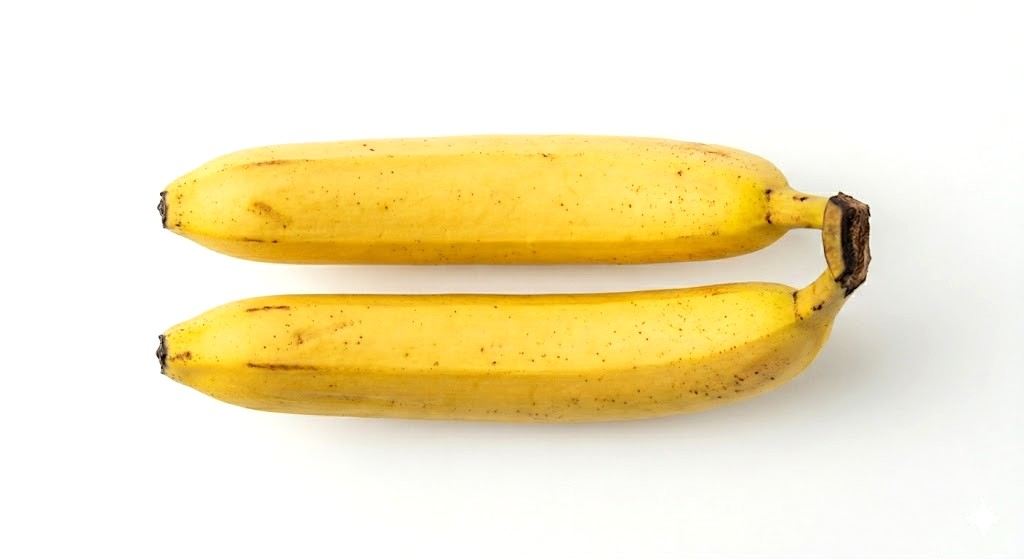
\includegraphics[width=\marginparwidth]{./figures/banana.jpg}
    \caption{Clustering allows us to move from a) and b) are similar to a) and b) are of the same. \textit{Image is generated with NanoBanana.}}
\end{marginfigure}

\newthought{In order to move from representation to leveraging pattern} we have good reason to find ways to,
\begin{itemize}
    \item compute partitions, of the data, given a distance measure.
    \item formalize what makes a well-defined partition by specifying an appropriate objective.
    \item recognize the geometric assumptions and finding ways to represent cluster characteristics.
\end{itemize}



\subsection{Hands On Experience}

\newthought{Consider} twelve data points in two dimensions.
Which points belong together? How many clusters do you see?

\begin{figure}
\centering
\begin{tikzpicture}[scale=1]
    \begin{axis}[
        xmin=0, xmax=10,
        ymin=0, ymax=10,
        width=0.5*\textwidth,
        height=0.5*\textwidth,
        axis line style={draw=none},
        tick style={black, thick},
        xtick={1,2,3,4,5,6,7,8,9},
        ytick={1,2,3,4,5,6,7,8,9},
        xticklabel style={font=\small},
        yticklabel style={font=\small},
        tick align=outside,
        tick pos=left,
    ]
    \addplot[only marks, mark=*, mark size=2pt, black] coordinates {
        (1,2) (2,1) (2,3) (3,2)
        (4,5) (5,4) (5,6) (6,5)
        (7,8) (8,7) (8,9) (9,8)
    };
    \end{axis}
\end{tikzpicture}
\caption{Twelve points in 2D. How many clusters do you see?}
\label{fig:intro_points}
\end{figure}

\newthought{How many clusters} do you see? Three seems natural, but could you argue for two?
For six? For 12?

\vspace{2.5em}
\newthought{Without ground truth}, there is no single right answer, as a context for any answer could be engineered. However, some answers are better than others, 
and it does not come as a surprise when I tell you that most people see three clusters in this data.


\newthought{The fundamental question} this chapter answers is how do we find the clusters mathematically? 
We will see how K-Means assigns each point to a cluster; and how cluster centroids function as representative points for each cluster.

\marginnote{\newthought{A centroid} is the mean position of all points assigned to a cluster.
It need not be an actual data point; it is the center of mass of the cluster.
The centroid exists in the same space as the data.
With a different distance, a different notion of center is needed.
For sake of simplicity and interpretability, we tie ourselves to Euclidean distance and arithmetic means.
But it is worth getting an intuition for other distances as well.}


\newthought{Where would you place} a representative point for each cluster?
Could you think of other measures to characterize and represent clusters, beyond a single point?


\newthought{The Learning Objectives} of this lecture:
\begin{itemize}
    \item Understand the K-Means objective and algorithm, including convergence.
    \item Apply initialization strategies and K-selection methods.
    \item Identify when K-Means fails and understand why.
\end{itemize}








% ==============================================================================================
% BLOCK 2: MAIN THEORY
% ==============================================================================================

\newpage

\section{The K-Means Algorithm}\index{K-Means}\index{inertia}

\newthought{A data point}\index{data point} is a vector $x_i \in \mathbb{R}^d$, where $d$ is the number of features and $i = 1, \ldots, n$ indexes the observations.

\begin{marginfigure}
    \centering
    \begin{tikzpicture}
        \begin{axis}[
            xmin=0, xmax=5,
            ymin=0, ymax=5,
            width=\marginparwidth,
            height=\marginparwidth,
            axis line style={draw=none},
            tick style={black, thin},
            xtick={1,2,3,4},
            ytick={1,2,3,4},
            xticklabel style={font=\tiny},
            yticklabel style={font=\tiny},
            tick align=outside,
            tick pos=left,
            xlabel={$x^{(1)}$},
            ylabel={$x^{(2)}$},
        ]
        \addplot[only marks, mark=*, mark size=2pt, black] coordinates {(3,2)};
        \node[font=\small, anchor=south west] at (axis cs:3.2,2.1) {$x_i$};
        \end{axis}
    \end{tikzpicture}
    \caption{A single data point $x_i$ in $\mathbb{R}^2$.}
\end{marginfigure}

\newthought{A cluster}\index{cluster} is a non-empty subset $C_k \subseteq \{x_1, \ldots, x_n\}$.
Each point belongs to exactly one cluster; this is the hard assignment assumption, meaning clusters are disjoint:

\begin{align*}
    C_j \cap C_k &= \emptyset \quad \text{for } j \neq k
\end{align*}

A clustering\index{clustering} of the data is a collection of $K$ clusters $\{C_1, \ldots, C_K\}$ that is exhaustive, every point is accounted for:

\begin{align*}
    \bigcup_{k=1}^{K} C_k &= \{x_1, \ldots, x_n\}
\end{align*}


\vspace{1.5em}
\marginnote{\newthought{Minimizing $J$} is NP-hard (effort exponential in $n$ and $K$) in general. K-Means finds a local optimum, not necessarily the global one. The result depends on initialization, and is thus non-deterministic. Shout out numerical methods.}
\newthought{K-Means} finds a clustering of $n$ data points into $K$ clusters by minimizing the total squared distance from each point to its cluster's centroid.
This quantity is called inertia or within-cluster sum of squares (WCSS):

\begin{align}
    J &= \sum_{k=1}^{K} \sum_{x_i \in C_k} \|x_i - \mu_k\|^2
    \label{eq:inertia}
\end{align}

where the mean $\mu_k = \frac{1}{|C_k|} \sum_{x_i \in C_k} x_i$ is the centroid of cluster $C_k$.

\begin{marginfigure}
    \centering
    \begin{tikzpicture}
        \begin{axis}[
            xmin=0, xmax=5,
            ymin=0, ymax=5,
            width=\marginparwidth,
            height=\marginparwidth,
            axis line style={draw=none},
            tick style={black, thin},
            xtick={1,2,3,4},
            ytick={1,2,3,4},
            xticklabel style={font=\tiny},
            yticklabel style={font=\tiny},
            tick align=outside,
            tick pos=left,
            xlabel={$x^{(1)}$},
            ylabel={$x^{(2)}$},
        ]
        \addplot[only marks, mark=*, mark size=2pt, black] coordinates {(1,3) (3,2) (4,3)};
        \node[font=\tiny, anchor=south east] at (axis cs:0.9,3.1) {$x_1$};
        \node[font=\tiny, anchor=north] at (axis cs:3,1.8) {$x_2$};
        \node[font=\tiny, anchor=south west] at (axis cs:4.1,3.1) {$x_3$};
        \draw[black!50, dotted, thick] (axis cs:1,3) -- (axis cs:2.67,2.67);
        \draw[black!50, dotted, thick] (axis cs:3,2) -- (axis cs:2.67,2.67);
        \draw[black!50, dotted, thick] (axis cs:4,3) -- (axis cs:2.67,2.67);
        \addplot[only marks, mark=o, mark size=2pt, black, thick] coordinates {(2.67,2.67)};
        \node[font=\tiny, anchor=south west] at (axis cs:2.87,2.8) {$\mu_k$};
        \end{axis}
    \end{tikzpicture}
    \caption{Cluster $C_k = \{x_1, x_2, x_3\}$ with centroid $\mu_k$. Dotted lines show the distances whose squares sum to $J$.}
    \label{fig:centroid}
\end{marginfigure}


\vspace{1.5em}
\newthought{The algorithm alternates between two steps} until the assignments no longer change. 
\marginnote{\newthought{Standard Algorithmic Form} was described by Lloyd\cite{Lloyd1982}}
It remains one of the most cited algorithms in machine learning, in part because it is easy to implement, easy to interpret, and fast enough to run on large datasets.



\begin{algorithm}[H]
\caption{K-Means}
\begin{algorithmic}[1]
\Require Data $X = \{x_1, \ldots, x_n\}$, number of clusters $K$, initial centroids $\mu_1, \ldots, \mu_K$
\Ensure Clustering $\{C_1, \ldots, C_K\}$, centroids $\{\mu_1, \ldots, \mu_K\}$
\Repeat
    \State \textbf{Assignment:} $c_i \leftarrow \arg\min_k \|x_i - \mu_k\|^2$ for each $x_i$
    \State \textbf{Update:} $\mu_k \leftarrow \frac{1}{|C_k|} \sum_{x_i:\, c_i = k} x_i$ for each $k$
\Until{assignments no longer change}
\end{algorithmic}
\end{algorithm}



\newthought{A trace through the algorithm} on three points with $K{=}2$ makes this concrete.
With initial centroids at $\mu_1{=}x_1{=}(1,3)$ and $\mu_2{=}x_3{=}(4,3)$:

\begin{itemize}
    \item For each point, the assignment step asks: which centroid is closest?
    \item For each cluster, the update step asks: given the current assignments, where is the new centroid?
\end{itemize}


\newthought{Step 1: Initialization.} We place two centroids at $\mu_1 = (1,4)$ and $\mu_2 = (4,1)$, away from any data point.

\begin{figure}
\centering
\begin{tikzpicture}
    \begin{axis}[
        xlabel={$x^{(1)}$}, ylabel={$x^{(2)}$},
        xmin=0, xmax=5, ymin=0, ymax=5,
        width=0.5\textwidth, height=0.5\textwidth,
        axis line style={draw=none},
        tick style={black, thin},
        xtick={1,2,3,4}, ytick={1,2,3,4},
        xticklabel style={font=\small},
        yticklabel style={font=\small},
        tick align=outside, tick pos=left,
    ]
    \addplot[only marks, mark=*, mark size=2pt, black!30] coordinates {(1,3)(3,2)(4,3)};
    \addplot[only marks, mark=o, mark size=2pt, black, thick] coordinates {(1,4)(4,1)};
    \node[font=\small, anchor=south east] at (axis cs:0.8,4.2) {$\mu_1$};
    \node[font=\small, anchor=north west] at (axis cs:4.2,0.8) {$\mu_2$};
    \end{axis}
\end{tikzpicture}
\caption{Initialization: two centroids placed away from the data. All points are unassigned.}
\label{fig:trace_init}
\end{figure}

\newthought{Step 2: Assignment.} Each point joins the cluster of its nearest centroid.
\begin{align*}
    x_1{=}(1,3)\!: \quad d^2(\mu_1) &= 0 + 1 = 1, \quad d^2(\mu_2) = 9 + 4 = 13 \;\to\; C_1 \\
    x_2{=}(3,2)\!: \quad d^2(\mu_1) &= 4 + 4 = 8, \quad d^2(\mu_2) = 1 + 1 = 2 \;\to\; C_2 \\
    x_3{=}(4,3)\!: \quad d^2(\mu_1) &= 9 + 1 = 10, \quad d^2(\mu_2) = 0 + 4 = 4 \;\to\; C_2
\end{align*}

\begin{figure}
\centering
\begin{tikzpicture}
    \begin{axis}[
        xlabel={$x^{(1)}$}, ylabel={$x^{(2)}$},
        xmin=0, xmax=5, ymin=0, ymax=5,
        width=0.5\textwidth, height=0.5\textwidth,
        axis line style={draw=none},
        tick style={black, thin},
        xtick={1,2,3,4}, ytick={1,2,3,4},
        xticklabel style={font=\small},
        yticklabel style={font=\small},
        tick align=outside, tick pos=left,
    ]
    \addplot[only marks, mark=*, mark size=2pt, black] coordinates {(1,3)};
    \addplot[only marks, mark=*, mark size=2pt, black!55] coordinates {(3,2)(4,3)};
    \addplot[only marks, mark=o, mark size=2pt, black, thick] coordinates {(1,4)(4,1)};
    \node[font=\small, anchor=south east] at (axis cs:0.8,4.2) {$\mu_1$};
    \node[font=\small, anchor=north west] at (axis cs:4.2,0.8) {$\mu_2$};
    \node[font=\small, anchor=north] at (axis cs:1,2.7) {$C_1$};
    \node[font=\small, anchor=north] at (axis cs:3.5,1.7) {$C_2$};
    \end{axis}
\end{tikzpicture}
\caption{Assignment: $x_1 \to C_1$ (dark), $x_2$ and $x_3 \to C_2$ (grey).}
\label{fig:trace_assign}
\end{figure}

\newthought{Step 3: Update.} Each centroid moves to the mean of its cluster.
\begin{align*}
    \mu_1' &= x_1 = (1,\; 3) \\
    \mu_2' &= \tfrac{1}{2}\bigl((3,2) + (4,3)\bigr) = (3.5,\; 2.5)
\end{align*}

\begin{figure}
\centering
\begin{tikzpicture}
    \begin{axis}[
        xlabel={$x^{(1)}$}, ylabel={$x^{(2)}$},
        xmin=0, xmax=5, ymin=0, ymax=5,
        width=0.5\textwidth, height=0.5\textwidth,
        axis line style={draw=none},
        tick style={black, thin},
        xtick={1,2,3,4}, ytick={1,2,3,4},
        xticklabel style={font=\small},
        yticklabel style={font=\small},
        tick align=outside, tick pos=left,
    ]
    \addplot[only marks, mark=*, mark size=2pt, black] coordinates {(1,3)};
    \addplot[only marks, mark=*, mark size=2pt, black!55] coordinates {(3,2)(4,3)};
    \addplot[only marks, mark=o, mark size=2pt, black, thick] coordinates {(1,3)(3.5,2.5)};
    % Arrows showing centroid movement
    \draw[->, black!40, thick] (axis cs:1,3.9) -- (axis cs:1,3.15);
    \draw[->, black!40, thick] (axis cs:4,1.1) -- (axis cs:3.6,2.4);
    \node[font=\small, anchor=south east] at (axis cs:0.8,3.2) {$\mu_1'$};
    \node[font=\small, anchor=south west] at (axis cs:3.7,2.6) {$\mu_2'$};
    \end{axis}
\end{tikzpicture}
\caption{Update: both centroids move (arrows). $\mu_1$ drops from $(1,4)$ to $(1,3)$; $\mu_2$ jumps from $(4,1)$ to $(3.5, 2.5)$. Re-running assignment yields the same clusters: converged.}
\label{fig:trace_update}
\end{figure}


\newthought{Convergence} is guaranteed in finite steps.
The argument rests on three observations:
first, each assignment step can only decrease $J$, since every point moves to an equal or closer centroid;
second, each update step can only decrease $J$, since the mean minimizes squared distance to its members;
third, there are at most $K^n$ possible assignment configurations.
Since $J$ is non-increasing and the number of states is finite, the algorithm must reach a fixed assignment and stop.

\marginnote{\newthought{Local optimum.} Convergence does not mean the algorithm found the best clustering. It found a clustering. A different initialization may yield a better one.}
Typical convergence takes 10--100 iterations in practice.



\vspace{2.5em}
\newthought{Initialization Matters}\index{K-Means++}

K-Means is sensitive to where centroids start.
If two initial centroids fall inside the same natural cluster, one cluster gets split and another gets merged, and the algorithm may never recover.

\begin{figure}
\centering
\begin{tikzpicture}[scale=1]
    % Good initialization result
    \begin{axis}[
        name=good,
        title={Good initialization: $J=3$},
        xlabel={$x_1$}, ylabel={$x_2$},
        xmin=0, xmax=10, ymin=0, ymax=10,
        width=0.45\textwidth, height=0.45\textwidth,
        axis line style={draw=none},
        tick style={black, thin},
        xtick={2,5,8}, ytick={2,5,8},
        xticklabel style={font=\small},
        yticklabel style={font=\small},
        tick align=outside, tick pos=left,
        title style={font=\small},
    ]
    \addplot[only marks, mark=*, mark size=2pt, black] coordinates {(1,2)(2,1)};
    \addplot[only marks, mark=*, mark size=2pt, black!55] coordinates {(4,5)(5,4)};
    \addplot[only marks, mark=*, mark size=2pt, black!20] coordinates {(8,9)(9,8)};
    \addplot[only marks, mark=x, mark size=6pt, black, thick] coordinates {(1.5,1.5)(4.5,4.5)(8.5,8.5)};
    \end{axis}

    % Bad initialization result
    \begin{axis}[
        name=bad,
        at={(good.east)}, anchor=west, xshift=0.8cm,
        title={Bad initialization: $J=34$},
        xlabel={$x_1$},
        xmin=0, xmax=10, ymin=0, ymax=10,
        width=0.45\textwidth, height=0.45\textwidth,
        axis line style={draw=none},
        tick style={black, thin},
        xtick={2,5,8}, ytick={2,5,8},
        xticklabel style={font=\small},
        yticklabel style={font=\small},
        tick align=outside, tick pos=left,
        title style={font=\small},
    ]
    % A is its own singleton cluster
    \addplot[only marks, mark=*, mark size=2pt, black] coordinates {(1,2)};
    % B is its own singleton cluster
    \addplot[only marks, mark=*, mark size=2pt, black!55] coordinates {(2,1)};
    % C, D, E, F all merged into one cluster
    \addplot[only marks, mark=*, mark size=2pt, black!20] coordinates {(4,5)(5,4)(8,9)(9,8)};
    \addplot[only marks, mark=x, mark size=6pt, black, thick] coordinates {(1,2)(2,1)(6.5,6.5)};
    \end{axis}
\end{tikzpicture}
\caption{Same data, different initial centroids. Left: one centroid per natural cluster gives $J{=}3$. Right: two centroids inside the same cluster leave the other two clusters merged, giving $J{=}34$.}
\label{fig:kmeans_init}
\end{figure}

\marginnote{\newthought{Multiple restarts.} A practical fix: run K-Means $n$ times with different random initializations, keep the result with the lowest $J$. Typical default: $n{=}10$.}

\newthought{K-Means++}\cite{ArthurVassilvitskii2007} gives a smarter starting point.
The first centroid is chosen uniformly at random.
Each subsequent centroid is chosen with probability proportional to its squared distance to the nearest already-chosen centroid:

\begin{align*}
    p(x_i) &= \frac{D(x_i)^2}{\sum_j D(x_j)^2}
\end{align*}

where $D(x_i) = \min_{j < k} \|x_i - \mu_j\|$.
Points far from all current centroids are more likely to be chosen next, spreading the initial centroids across the data.
This gives a theoretical guarantee on the expected inertia relative to the global optimum.



\vspace{2.5em}
\newthought{Choosing K}\index{elbow method}\index{silhouette score}

K must be set by the practitioner.
Two complementary heuristics help.

\newthought{The elbow method} plots inertia $J$ against $K$ and looks for a kink: the point where adding one more cluster yields diminishing returns.
For our six points, $J$ drops sharply from $K{=}1$ to $K{=}3$, then flattens.

\begin{figure}
\centering
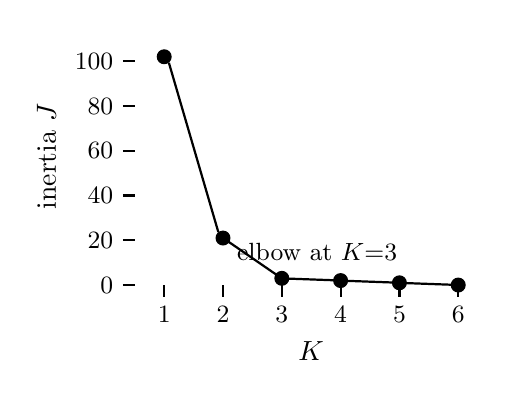
\begin{tikzpicture}[scale=1]
    \begin{axis}[
        xlabel={$K$},
        ylabel={inertia $J$},
        xmin=0.5, xmax=6.5,
        ymin=0, ymax=115,
        width=0.5*\textwidth,
        height=0.4*\textwidth,
        axis line style={draw=none},
        tick style={black, thick},
        xtick={1,2,3,4,5,6},
        ytick={0,20,40,60,80,100},
        xticklabel style={font=\small},
        yticklabel style={font=\small},
        tick align=outside,
        tick pos=left,
    ]
    % Dots only
    \addplot[only marks, mark=*, mark size=2.5pt, black] coordinates {
        (1,102) (2,21) (3,3) (4,2) (5,1) (6,0)
    };
    % Line segments with gaps near each dot (Tufte style)
    \draw[black, thick] (axis cs:1.08,99.3) -- (axis cs:1.92,23.7);
    \draw[black, thick] (axis cs:2.08,19.6) -- (axis cs:2.92,4.4);
    \draw[black, thick] (axis cs:3.08,2.9) -- (axis cs:3.92,2.1);
    \draw[black, thick] (axis cs:4.08,1.9) -- (axis cs:4.92,1.1);
    \draw[black, thick] (axis cs:5.08,0.9) -- (axis cs:5.92,0.1);
    \draw[black!40, dashed] (axis cs:3,3) -- (axis cs:3,0);
    \node[font=\small] at (axis cs:3.6,15) {elbow at $K{=}3$};
    \end{axis}
\end{tikzpicture}
\caption{Elbow plot for the six sample points. The kink at $K{=}3$ matches the three natural clusters.}
\label{fig:elbow}
\end{figure}

\marginnote{\newthought{The elbow is not always clear.} On real data, the curve may decrease smoothly with no obvious kink. The elbow is a heuristic, not a guarantee.}

\newthought{The silhouette score}\index{silhouette score} measures how well each point fits its assigned cluster relative to the next-best cluster.
For point $x_i$, let $a(i)$ be its mean distance to points in the same cluster and $b(i)$ its mean distance to points in the nearest other cluster:

\begin{align*}
    s(i) &= \frac{b(i) - a(i)}{\max\bigl(a(i),\, b(i)\bigr)}
\end{align*}

$s(i)$ ranges from $-1$ (point would fit better elsewhere) to $+1$ (point is well-placed).
The mean silhouette over all points is a quality score for the full clustering.
Choose $K$ that maximizes it.

\marginnote{\newthought{For our six points} with $K{=}3$, every point has $a(i) {=} \sqrt{2} \approx 1.4$ and $b(i) \approx 4.4$, giving $s(i) \approx 0.68$. A clear, well-separated clustering.}



\vspace{2.5em}
\newthought{When K-Means Fails}\index{failure modes}

K-Means assumes clusters are roughly spherical, equally sized, and equally dense.
When the data violates these assumptions, the Voronoi partition imposed by Euclidean centroids cuts the data in the wrong places.

\begin{figure}
\centering
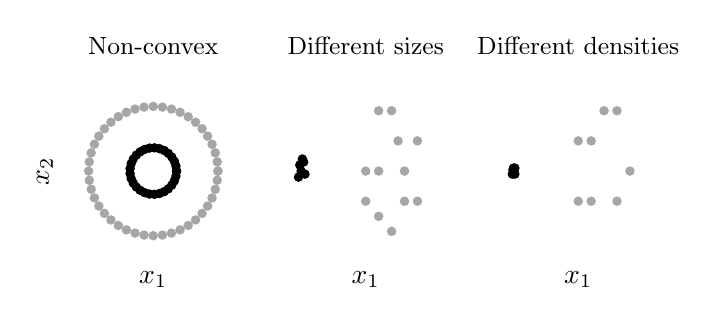
\begin{tikzpicture}[scale=1]
    % Panel 1: Non-convex (rings)
    \begin{axis}[
        name=rings,
        title={Non-convex},
        xlabel={$x_1$}, ylabel={$x_2$},
        xmin=-3.5, xmax=3.5,
        ymin=-3.5, ymax=3.5,
        width=0.32\textwidth, height=0.32\textwidth,
        axis line style={draw=none},
        tick style={draw=none},
        xtick=\empty, ytick=\empty,
        title style={font=\small},
        axis equal,
    ]
    \addplot[only marks, mark=*, mark size=1.5pt, black,
        domain=0:360, samples=30] ({0.9*cos(x)}, {0.9*sin(x)});
    \addplot[only marks, mark=*, mark size=1.5pt, black!35,
        domain=0:360, samples=45] ({2.5*cos(x)}, {2.5*sin(x)});
    \end{axis}

    % Panel 2: Different sizes
    \begin{axis}[
        name=sizes,
        at={(rings.east)}, anchor=west, xshift=0.4cm,
        title={Different sizes},
        xlabel={$x_1$},
        xmin=-2, xmax=12,
        ymin=-3, ymax=3,
        width=0.32\textwidth, height=0.32\textwidth,
        axis line style={draw=none},
        tick style={draw=none},
        xtick=\empty, ytick=\empty,
        title style={font=\small},
    ]
    \addplot[only marks, mark=*, mark size=1.5pt, black] coordinates {
        (0,0)(0.2,0.3)(-0.1,0.2)(0.3,-0.1)(-0.2,-0.2)(0.1,0.4)
    };
    \addplot[only marks, mark=*, mark size=1.5pt, black!35] coordinates {
        (6,0)(7.5,1)(8,0)(6,-1.5)(7,-2)(9,1)(5,0)(8,-1)(6,2)(9,-1)(7,2)(5,-1)
    };
    \end{axis}

    % Panel 3: Different densities
    \begin{axis}[
        name=densities,
        at={(sizes.east)}, anchor=west, xshift=0.4cm,
        title={Different densities},
        xlabel={$x_1$},
        xmin=-2, xmax=12,
        ymin=-2, ymax=4,
        width=0.32\textwidth, height=0.32\textwidth,
        axis line style={draw=none},
        tick style={draw=none},
        xtick=\empty, ytick=\empty,
        title style={font=\small},
    ]
    \addplot[only marks, mark=*, mark size=1.5pt, black] coordinates {
        (0,1)(0.1,0.9)(0,1.1)(0.05,0.95)(-0.05,1.05)(0.1,1.1)(-0.1,0.9)
    };
    \addplot[only marks, mark=*, mark size=1.5pt, black!35] coordinates {
        (5,0)(8,3)(6,0)(9,1)(5,2)(8,0)(7,3)(6,2)
    };
    \end{axis}
\end{tikzpicture}
\caption{Three scenarios where K-Means fails. Left: concentric rings share a centroid and cannot be separated. Centre: a large and a small cluster pull the boundary toward the small one. Right: a dense and a sparse cluster of equal inertia look equivalent to K-Means.}
\label{fig:kmeans_failures}
\end{figure}

\marginnote{\newthought{K-Medoids} uses actual data points as cluster centers instead of means, making it robust to outliers and compatible with non-Euclidean distances. \newthought{Mini-Batch K-Means} updates centroids on random subsets of the data, scaling to millions of points at the cost of a slightly noisier result.}

\newthought{When K-Means struggles}, the underlying issue is always the same: the Euclidean distance to a centroid is the wrong measure of belonging for that data.
The next chapters address this by changing the notion of neighborhood (hierarchical clustering) and of density (DBSCAN).



% ==============================================================================================
% BLOCK 3: STUDENT ACTIVATION
% ==============================================================================================

\newpage

\section{Examples \& Exercises}\index{examples}\index{exercises}

\marginnote{\newthought{Exercises} are for practice and reinforcing concepts. Try to solve them on your own first,
try things, play with it, discuss; this is not a time trial. And there is no shame in not ending up at the right answer,
in the same sense that uncovering great questions
and tossing them around is usually pretty fruitful in the long run.}

\newthought{Computing by hand} builds the intuition that no amount of library calls can replace.
Step through the arithmetic slowly.

\vspace{1em}

\marginnote{$A=(1,2)$, $B=(2,1)$\\$C=(4,5)$, $D=(5,4)$\\$E=(8,9)$, $F=(9,8)$\\[4pt]acidity, bitterness (1--10)}
\newthought{Given six coffee samples} $A$--$F$, run K-Means with $K{=}3$ and initial centroids $\mu_1{=}A$, $\mu_2{=}C$, $\mu_3{=}E$.
Perform the assignment step, the update step, and compute the inertia after convergence.

\vspace{0.5em}

The assignment step computes the squared distance from each point to each centroid and assigns each point to the nearest one.
The distances are symmetric by construction so we only check whether a point is closest to its natural cluster center:

\begin{align*}
    d(A,\mu_1)^2 &= 0, \quad d(A,\mu_2)^2 = 18, \quad d(A,\mu_3)^2 = 98 \;\to\; C_1 \\
    d(B,\mu_1)^2 &= 2, \quad d(B,\mu_2)^2 = 20, \quad d(B,\mu_3)^2 = 100 \;\to\; C_1 \\
    d(C,\mu_1)^2 &= 18, \quad d(C,\mu_2)^2 = 0, \quad d(C,\mu_3)^2 = 32 \;\to\; C_2 \\
    d(D,\mu_1)^2 &= 20, \quad d(D,\mu_2)^2 = 2, \quad d(D,\mu_3)^2 = 34 \;\to\; C_2 \\
    d(E,\mu_1)^2 &= 98, \quad d(E,\mu_2)^2 = 32, \quad d(E,\mu_3)^2 = 0 \;\to\; C_3 \\
    d(F,\mu_1)^2 &= 100, \quad d(F,\mu_2)^2 = 34, \quad d(F,\mu_3)^2 = 2 \;\to\; C_3
\end{align*}

The update step recomputes each centroid as the mean of its assigned points:

\begin{align*}
    \mu_1' &= \tfrac{1}{2}\bigl((1,2)+(2,1)\bigr) = (1.5,\;1.5) \\
    \mu_2' &= \tfrac{1}{2}\bigl((4,5)+(5,4)\bigr) = (4.5,\;4.5) \\
    \mu_3' &= \tfrac{1}{2}\bigl((8,9)+(9,8)\bigr) = (8.5,\;8.5)
\end{align*}

Running the assignment step again with the new centroids yields the same clusters; the algorithm has converged.
The inertia is:

\begin{align*}
    J &= \|A - \mu_1'\|^2 + \|B - \mu_1'\|^2
       + \|C - \mu_2'\|^2 + \|D - \mu_2'\|^2
       + \|E - \mu_3'\|^2 + \|F - \mu_3'\|^2 \\
      &= 0.5 + 0.5 + 0.5 + 0.5 + 0.5 + 0.5 \\
      &= 3
\end{align*}

Each pair contributes equally; the clustering is geometrically symmetric.


\vspace{2.5em}
\newthought{Now repeat} with bad initial centroids $\mu_1{=}A$, $\mu_2{=}B$, $\mu_3{=}C$ — two centroids inside the cold-brew cluster.

\marginnote{\newthought{What goes wrong.} Both $\mu_1$ and $\mu_2$ compete for cold-brew samples. The algorithm optimizes what it is given; it has no way of knowing that $A$ and $B$ are in the same natural cluster.}

Assignment step with $\mu_1{=}(1,2)$, $\mu_2{=}(2,1)$, $\mu_3{=}(4,5)$:

\begin{align*}
    A &\to C_1 \quad (\text{distance 0 to } \mu_1) \\
    B &\to C_2 \quad (\text{distance 0 to } \mu_2) \\
    C,\,D,\,E,\,F &\to C_3 \quad (\text{all closer to } \mu_3 \text{ than to } \mu_1 \text{ or } \mu_2)
\end{align*}

After the update: $\mu_1{=}(1,2)$ (singleton), $\mu_2{=}(2,1)$ (singleton), $\mu_3{=}(6.5,6.5)$ (four points merged).
The assignments do not change in the next iteration.
The inertia of this converged solution is:

\begin{align*}
    J_{\text{bad}} &= 0 + 0 + \|C - \mu_3\|^2 + \|D - \mu_3\|^2 + \|E - \mu_3\|^2 + \|F - \mu_3\|^2 \\
                   &= 0 + 0 + 8.5 + 8.5 + 8.5 + 8.5 \;=\; 34
\end{align*}

The bad initialization found a solution more than ten times worse than the good one ($J{=}34$ vs $J{=}3$).
This is why K-Means++ and multiple restarts matter.


\vspace{2.5em}
\newthought{For the elbow method}, run K-Means on the same six points for $K = 1, \ldots, 6$ and record the inertia.

\marginnote{Inertia values:\\[4pt]
\begin{tabular}{cc}
$K$ & $J$ \\
\hline
1 & 102 \\
2 & 21 \\
3 & 3 \\
4 & 2 \\
5 & 1 \\
6 & 0 \\
\end{tabular}}

The drop from $K{=}1$ to $K{=}3$ is large (102 to 3); from $K{=}3$ onward the curve is nearly flat.
The elbow is at $K{=}3$, matching the three natural coffee varieties.
Note that $K{=}6$ always achieves $J{=}0$ by placing one centroid per point; this is not useful.



% ============================= CODE ===============================
\marginnote{\newthought{Code} will be provided as a Python notebook. Use it as a starting point, break things, and observe what changes.}

\marginnote{$n=20$ samples\\
\textit{acidity} (1--10)\\
\textit{bitterness} (1--10)\\[4pt]
Varieties: cold brew, drip, espresso, latte.}
\newthought{A coffee dataset to explore.} Load the dataset and scatter-plot acidity vs.\ bitterness.
Run K-Means with $K{=}3$ on raw features and visualize the cluster assignments.
Try different random seeds; how stable are the results?
Then vary $K$ from 1 to 8, record the inertia and silhouette score for each, and plot both curves.
Finally, deliberately give K-Means a bad initialization and compare the resulting inertia with the K-Means++ result.

\newthought{What to observe.} With a good initialization and $K{=}3$, the three clear clusters emerge immediately.
The elbow and the silhouette peak agree at $K{=}3$.
With a bad initialization, inertia is higher and cluster boundaries shift; the silhouette score drops.
With $K{=}4$ a natural cluster splits in two, and the silhouette score begins to fall.



\section{Self-Reflection and Recap}\index{reflection}\index{recap}

\newthought{Self-Reflection} questions to guide your thinking:
\begin{itemize}
    \item What does the K-Means objective actually minimize, and why is that a reasonable definition of a good clustering?
    \item Why does K-Means always converge, and why does convergence not guarantee the best solution?
    \item What does K-Means++ change about the initialization, and why does spreading centroids out help?
    \item When would you trust the elbow method? When would you not?
    \item How does the silhouette score measure something different from inertia?
    \item What shape of cluster cannot K-Means find, and why?
    \item How does the choice of distance metric interact with the K-Means update step?
    \item Given a new dataset, what would be your first three steps before running K-Means?
\end{itemize}

\newthought{Recap} of Key Concepts:
\begin{itemize}
    \item K-Means minimizes inertia by alternating assignment (points to nearest centroid) and update (centroid to cluster mean)
    \item Convergence is guaranteed; optimality is not, use K-Means++ or multiple restarts
    \item The elbow and silhouette score are complementary heuristics for choosing $K$
    \item K-Means assumes spherical, equally sized clusters; it fails on rings, elongated shapes, and density differences
\end{itemize}

\marginnote{\newthought{Teaser.} K-Means assigns every point to exactly one flat cluster. What if structure exists at multiple scales, or if some points genuinely belong between clusters?}
\newthought{So far, we found flat partitions} of the data into $K$ fixed clusters.
But natural structure is often hierarchical: coffee varieties cluster by roast, roasts cluster by origin, origins cluster by continent.
And some points genuinely sit at the boundary of two clusters, which a hard assignment hides.
The next chapters address both: hierarchical clustering reveals nested structure through dendrograms, and density-based methods find clusters of arbitrary shape without requiring a fixed $K$.
